%% Full length research paper template
%% Created by Simon Hengchen and Nilo Pedrazzini for the Journal of Open Humanities Data (https://openhumanitiesdata.metajnl.com)

\documentclass[11pt]{article}
\usepackage[english]{babel}
\usepackage[utf8]{inputenc}
\usepackage{johd}

\usepackage[margin=3cm]{geometry}
\usepackage{algpseudocode}
\usepackage{algorithm}
\usepackage{algorithmic}

\usepackage{amsthm}
\theoremstyle{definition}
\newtheorem{definition}{Definition}[section]

\begin{document}
\begin{center}
    \huge{Christian-Albrechts-Universität zu Kiel} \\[10pt]
    \large{Institut für Informatik}\\[40pt]
\end{center}

\begin{figure}[H]
\centering

\includegraphics[scale=0.7]{images/faculty.png}\\[40pt]
\end{figure}
\begin{center}
    \huge{Master Thesis} \\[10pt]
    \textbf{ „What’s between ‚em?“ - An approach for detecting in-between class instances}\\[10pt]
    \text{Md Abu Noman Majumdar}\\[20pt]
\end{center}

\begin{center}
    \large{Betreuer:}\\[10pt]
    \text{\Large Prof. Dr. Peer Kroeger}\\[10pt]
    \text{Zweitbetreuer}\\[10pt]
    \text{\Large Daniyal Kazempour}\\[10pt]
     Christian-Albrechts-Universität zu Kiel\\
     Institut für Informatik\\
     Wirtschaftsinformatik (Angewandte Informatik)\\
     Olshausenstr. 40, 24098 Kiel\\[10pt]
     \Large{February 2023}\\[50pt]
\end{center}

\newpage
\begin{abstract} 
\noindent Objects surrounded by classes/clusters and why that metters. In this paper, we propose a formulation for detect an object in between clusters witch can carry important information by witch we can find  relation among cluster that is based on the distance of a point from its $k^{th}$  nearest neighbor. First to find an outlier we have implemented hierarchical clustering method. After that we have defined a threshold to obtain outliers. After having outlier we have mined $k^{th}$ nearest cluster by considering euclidean distance and cosine distance. To be more accurate we have further considered a set of closest objects from each cluster to outlier so that we can prune clusters witch are behind of other cluster. This results in substantial savings in computation. We present the results of an extensive experimental study on real-life and synthetic data sets. The results from a real-life molecular data set highlight and reveal several expected and unexpected aspects of  clusters. The results from a study on synthetic data sets
demonstrate that the ....

\end{abstract}

\newpage

\tableofcontents

\newpage

\section{Introduction}
Unsupervised machine learning tasks like clustering and outlier detection are well known and accompanied by a rich body of literature. There are however cases in different domains where one is interested to identify objects that are 'enclosed' / 'in-between' several clusters/classes. This is of interest to identify objects that may share properties from different classes, hence embodying a bridge/connector.\\

 Outliers can sometimes be interesting observations because they may share properties with multiple classes or clusters, and can therefore act as "bridges" or "connectors" between different groups. In this case, it may be useful to treat the outlier as a special case and perform additional analysis to understand its unique characteristics and how it relates to the rest of the data. It's worth noting that not all outliers will be interesting or relevant to the analysis. Some outliers may simply be errors in the data that should be corrected or removed, while others may represent a completely different population and may not be relevant to the analysis. It's important to carefully evaluate the nature and significance of any outliers that are identified in the data.

 Identifying objects that may share properties from different classes and act as "bridges" or "connectors" between different groups can be a challenging task. One approach to finding such objects is to perform a clustering analysis and look for observations that are outliers or do not fit well into any of the clusters. These observations may be more likely to share properties with multiple classes and act as "bridges" between different groups. Another approach is to use a dimensionality reduction technique such as principal component analysis (PCA) or t-distributed stochastic neighbor embedding (t-SNE) to visualize the data in a lower-dimensional space. This can help identify observations that are "in between" different groups and may have characteristics that are shared across multiple classes. It's worth noting that finding objects that act as "bridges" between different groups can be a challenging and time-consuming task, and may require additional analysis and interpretation to fully understand their characteristics and how they relate to the rest of the data. \\
 
 In this paper we have tried to define an object in between several cluster
 
While the idea/intuition of an in-between instance may seem trivial, the truth reveals that one faces several open questions and challenges. To name some/a few ... [here can be your challenges ;-)  ]

To name a prominent example: while we may have a k-NN / 3rd-NN, the 3rd NN may not be of interest, since it is located "beyond" the 2nd NN, rendering it as a 'false' nearest neighbor in context of in-between instance detection.

\section{Related Work}
This section is dedicated to several open questions that may arise for the reader while dealing with the in-between instance problem. On the one hand, an overview of the outlier-detection landscape is sketched which we deem to be a 'relative' to the in-between instance detection problem followed by some elaborations on the fuzzy clustering archetype of algorithms. Alongside the listing of these methods, we also highlight the weaknesses/lacking characteristics/properties that ultimately lead/justify the need for the in-between instance problem.


\subsection{Outlier Detection}
An outlier is a data point that falls significantly outside the range of the majority of the data points in a dataset. Outliers can occur for a variety of reasons, such as errors in data collection or measurement, or they may indicate an unusual or unexpected event or phenomenon.

In statistical analysis, outliers can have a significant impact on the results of the analysis and the conclusions that are drawn. For example, they may cause the mean or median of a dataset to be distorted, or they may affect the results of statistical tests such as t-tests or ANOVA. As a result, it is often important to identify and analyze outliers carefully to understand their potential impact on the results of the analysis.

%dummy for citation:
The overall picture on outlier methods as elaborated on in \cite{outliersurvey}

There are several methods for identifying and analyzing outliers in statistical analysis. Some common methods include:\\

%some dummy suggestion:
\textit{Classification-based outlier detection}: Classification-based outlier detection methods involve training a classifier to distinguish between inliers (normal data points) and outliers. Once the classifier has been trained, it can be used to predict whether a new data point is an outlier or not. Classification-based outlier detection can be an effective method for identifying outliers in a dataset, particularly when the inlier and outlier data points are well-separated and easy to distinguish. However, it can be challenging to train a classifier to accurately distinguish between inliers and outliers, particularly when the inlier and outlier data points are not well-separated. Leaving the supervised realm there are outlier detections in the unsupervised setting as is elaborated below.\\


\textit{Clustering-based outlier detection}: Clustering-based outlier detection methods involve dividing the data points in a dataset into clusters, and then identifying data points that are significantly different from the other data points in their cluster. These data points are considered to be outliers.There are a variety of different clustering algorithms that can be used for outlier detection, including: K-means clustering, Density-based clustering, Hierarchical clustering Clustering-based outlier detection can be an effective method for identifying outliers in a dataset, particularly when the outliers are significantly different from the rest of the data points in some way (e.g., they are much larger or smaller, or have different characteristics). However, it can be challenging to determine the appropriate number of clusters to use and to tune the parameters of the clustering algorithm to achieve good results.Leaving the unsupervised realm there are outlier detections in the neural network setting as is elaborated below.\\


\textit{Neural network-based outlier detection}: Neural networks can be used for outlier detection by training a neural network to distinguish between normal data points (inliers) and anomalous data points (outliers). There are a few different approaches to using neural networks for outlier detection, including:

Autoencoders: An autoencoder is a type of neural network that is trained to reconstruct its input data. When an autoencoder is trained on inlier data points, it should be able to reconstruct those data points accurately. Outliers, on the other hand, may be difficult for the autoencoder to reconstruct, indicating that they are anomalous.

One-class classification: A neural network can be trained to perform one-class classification, where it is only trained on inlier data points and must distinguish between inliers and outliers.

Anomaly detection: A neural network can be trained to perform anomaly detection, where it is trained on both inlier and outlier data points and must distinguish between the two.

Using neural networks for outlier detection can be an effective method, particularly when the inliers and outliers have complex patterns that are difficult to capture with other methods. However, training a neural network can be computationally expensive and may require a large amount of labeled data.Leaving the neural network realm there are outlier detections in the probabilistic  setting as is elaborated below.\\

\textit{Bayesian networks-based outlier detection}:Bayesian networks are probabilistic graphical models that represent the dependencies between variables as a directed acyclic graph (DAG). Bayesian networks can be used for outlier detection by representing the data points in a dataset as variables in the network, and modeling the dependencies between the variables using a DAG. Outliers can then be identified as data points that have significantly different probabilities or dependencies compared to the other data points in the network.

One potential benefit of using Bayesian networks for outlier detection is that they can handle complex dependencies between variables and can incorporate prior knowledge about the relationships between variables. However, constructing a Bayesian network can be challenging, particularly when the number of variables is large or when the relationships between variables are not well-understood. In addition, Bayesian networks can be computationally expensive to work with, particularly when the network is large or the data is high-dimensional.\\



It is important to consider the context of the data and the potential causes of the outliers when interpreting the results of the analysis. Outliers may be caused by errors in data collection or measurement, or they may indicate an unusual or unexpected event or phenomenon that is worth further investigation.

\subsection{Fuzzy Clustering}
Fuzzy clustering, also known as fuzzy c-means clustering, is a machine learning technique used to group data points into clusters, where each data point can belong to more than one cluster with a degree of membership. This is in contrast to traditional clustering algorithms, which assign each data point to a single cluster.\\
The overall picture on Fuzzy Clustering methods as elaborated on in \cite{grover2014study}.
Fuzzy clustering is useful in situations where it is not clear which cluster a data point belongs to, or where the data points may belong to multiple clusters. It is often used in image and text classification, data mining, and other applications where there may be overlap or uncertainty in the data.

To perform fuzzy clustering, the data points are first randomly initialized into clusters, and the degree of membership of each data point in each cluster is calculated using a membership function. The membership function assigns a membership value between 0 and 1 to each data point, with a value of 1 indicating that the data point belongs fully to the cluster and a value of 0 indicating that it does not belong to the cluster at all.

The membership values are then used to update the centroids (representative points) of the clusters, and the process is repeated until the membership values and centroids converge to stable values. The final clusters are then formed by assigning each data point to the cluster with the highest membership value.

There are several variations of the fuzzy c-means algorithm, including the possibilistic c-means (PCM) algorithm and the modified PCM (MPCM) algorithm. These variations can be used to improve the accuracy and stability of the clustering process.

\subsection{In-between Instance Detection}
To detect in-between instances in a dataset that has been divided into clusters, we can use a variety of techniques, including:

Nearest neighbor algorithms: These algorithms identify the data points that are closest to the instance being classified, and use the class or label of those data points to predict the class or label of the instance.

Decision trees: Decision trees are used to classify instances based on their features or attributes. They work by building a tree-like model that splits the data into smaller and smaller groups based on the values of the features, until a decision can be made about the class or label of the instance.

Support vector machines (SVMs): SVMs are a type of supervised machine learning algorithm that can be used to classify in-between instances. They work by finding the hyperplane that maximally separates the different classes in the dataset, and then using that hyperplane to classify new instances.

Neural networks: Neural networks are a type of machine learning algorithm that can be used to classify in-between instances. They work by building a network of interconnected nodes, or artificial neurons, that can learn to recognize patterns in the data and make predictions based on those patterns.

It is important to carefully evaluate the performance of the algorithm used for in-between instance detection, as the accuracy of the predictions can have significant implications for the application being studied.

General "rule-of-thumb" 
a) state what the paper does in 2-3 sentences
b) state why that paper is not already the solution to what we need/what is "missing"
$\rightarrow$ "that is what we provide in this work"

\section{Main Method}

The approach to identify in-between instances is covered by several parts, as it is elaborated on in the following:

\subsection{What is an in-between instance, and how is it defined?}

\begin{definition}[In-between Instance]
Let there is a cluster set $D$ with cluster $d1,d2,d3,...,dn$ and also there is a outlier $O$. This outlier $O$ will be considered as an in-between instance if it surrounded by at least two cluster by excluding other cluster from $k$ nearest neighbor under the condition  where cosine distance between  outlier $o$ and cluster $d\text\textsc{k}$ is $>=1$ with respect to any other cluster as an origin.
\end{definition}

\begin{figure}[H]
\centering
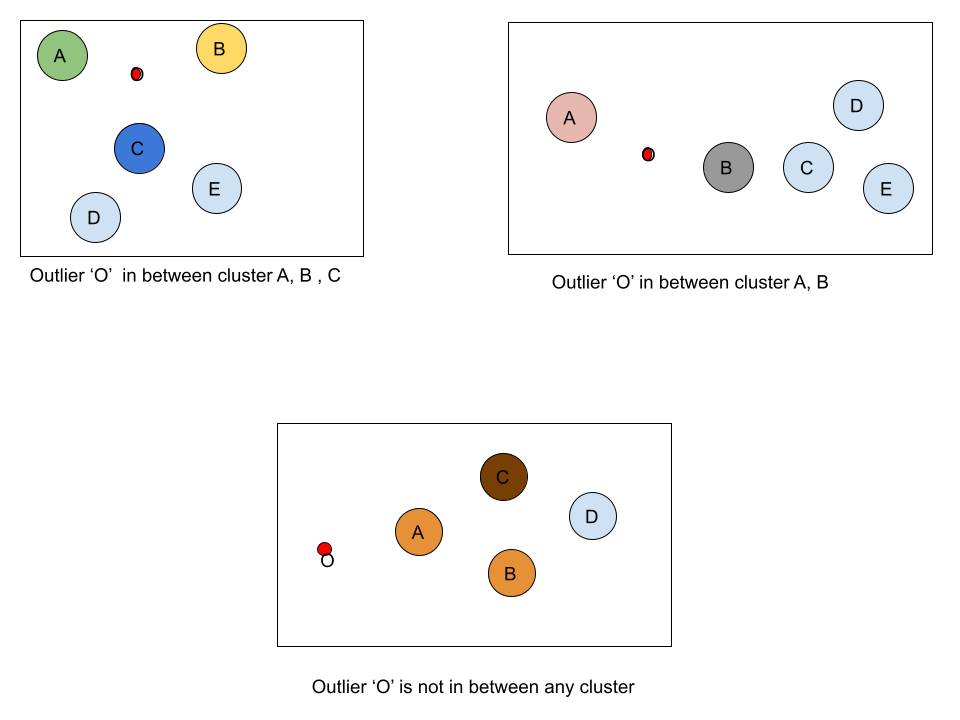
\includegraphics[scale=.4]{images/Object-in-btwn-cluster.png}\\
Figure: Object in between clusters
\end{figure}

\subsection{What is the in-between instance detection \textbf{task} and how is it defined?}

The task can be defined in 3 phases.\\
\textbf{First phase}:\\
First of all we need a collection of clusters and outliers of a data set. For that we have used \textbf{Agglomerative Hierarchical Clustering} because we can explicitly define the threshold distance to create a new cluster which is not possible in K-means clustering algorithm. First we have applied the agglomerative algorithm with no distance threshold and observe the dendrogram. \\

A dendrogram is a diagram that shows the hierarchical relationship between objects. It is most commonly created as an output from hierarchical clustering. The main use of a dendrogram is to work out the best way to allocate objects to clusters.After observing the dendrogram we defined the distance threshold. Then we again run agglomerative algorithm. As a result we have got a set of cluster where among them some cluster contain only few instances are recognized as outlier.\\

\noindent\textbf{Second phase}:\\
After having set of cluster and outlier we have computed the k-nearest neighbour of a particular outlier by applying euclidean distance.These K-nearest cluster will be further filtered to get precise neighbour clusters where the outlier will be in between them.\\


\noindent\textbf{Third phase}:\\
After having the k-nearest cluster for a particular outlier we have applied \textbf{In-between Instance} algorithm that we have defined is given below:  \\

\begin{algorithm}[hbt!]
\caption{ In-between Instance}\label{alg:cap}
\begin{algorithmic}[1]
\Require $ K\textunderscore NearestCluster(Distance, Outlier, Cluster),clusterMean[], Outlier$\\
\Ensure $[(inbetweenobject,[neighclust1, neighclust5,...]),(),...]$
\State $ closestCluster \gets K\textunderscore NearestCluster[0][2] $
\State $ closestDistance \gets K\textunderscore NearestCluster[0][0] $
\State $ candidateCluster \gets [] $
\State $ rejectedCluster \gets [] $
\State $ candidateCluster.append(K\textunderscore NearestCluster[0]) $

\For {$i$ in $K\textunderscore NearestCluster$ }  
    \State {
    \If{$i$ in $rejectedCluster$}
    $continue$
    \EndIf
    \For {$j$ in $K\textunderscore NearestCluster$ } 
        \State {
        \If{$i == j$}
        $continue$
        \EndIf
        %\State $ distanceBetween \gets %distance.euclidean(clusterMean[i[2]],clusterMean[j[2]]) $
        \State $ origin \gets clusterMean[i[2]] + (- clusterMean[i[2]]) $
        \State $ translateOutlier \gets clusterMean[i[1]] + (- clusterMean[i[2]]) $
        \State $ translateCluster \gets clusterMean[j[2]] + (- clusterMean[i[2]])$
        \State $ cosineDistance \gets distance.cosine(translateOutlier, translateCluster) $
        \If{$ cosineDistance < 1$}
            \State{
            \If{$j$ in $candidateCluster$}
                    continue
                \EndIf
                \State $candidateCluster.append(j)$
            }
            
        \Else 
            \State{
            \If{$j$ not in $rejectedCluster$}
                \State $rejectedCluster.append(j)$
                \EndIf
                \If{$j$ not in $candidateCluster$}
                \State $candidateCluster.remove(j)$
                \EndIf
            }
            \\
        \EndIf
        }
    \EndFor
    }
\EndFor
\For{$i$ in $candidateCluster$}
    \If{$i$ in $rejectedCluster$}
        \State $candidateCluster.remove(i)$
    \EndIf
\EndFor 
\\
\algorithmicreturn{ $candidateCluster $} 


\end{algorithmic}
\end{algorithm}
\newpage
\noindent In this algorithm we have provided three inputs. One is a list of tuples that we have called 'K-Nearest-Cluster'. The tuple consists of distance, outlier, and cluster where distance is the euclidean distance between outlier and cluster mean. Another input is a list of cluster mean and the last input is an outlier. As output, we are expecting the same list of tuples where it will contain only those clusters that satisfy our 'In-between Instance' definition. If our output list contains only a single element then we will consider our outlier as a not-in-between instance.\\

\noindent According to the definition we have iterated over all clusters which we can see in our algorithm from lines 9 to 35. Each time of iteration we again iterate all clusters except the own cluster from the first iteration which is executed from lines 11 to 34. In the second iteration loop for a cluster, we have translated the coordinate to the origin. That's why we have translated other related elements according to the new origin which is implemented from lines 15 to 17.  A translation is a slide from one location to another, without any change in size or orientation.
\begin{figure}[H]
\centering
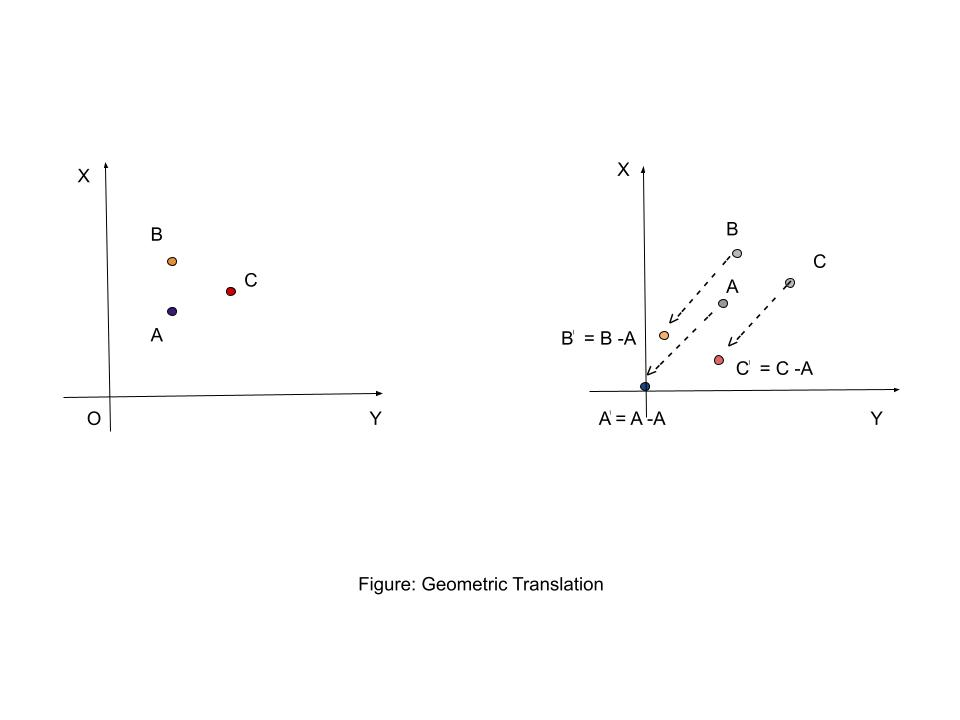
\includegraphics[scale=.4]{images/Geometric-translation.jpg}\\
Figure: Object in between clusters
\end{figure}
\noindent After translating the cluster to the origin we  have calculated the cosine distance between the outlier and other clusters with respect to the cluster that was translated to the origin. if the cosine distance is greater than 1 we have discarded those clusters from the candidate cluster list because they are behind of other clusters.

\begin{figure}[H]
\centering
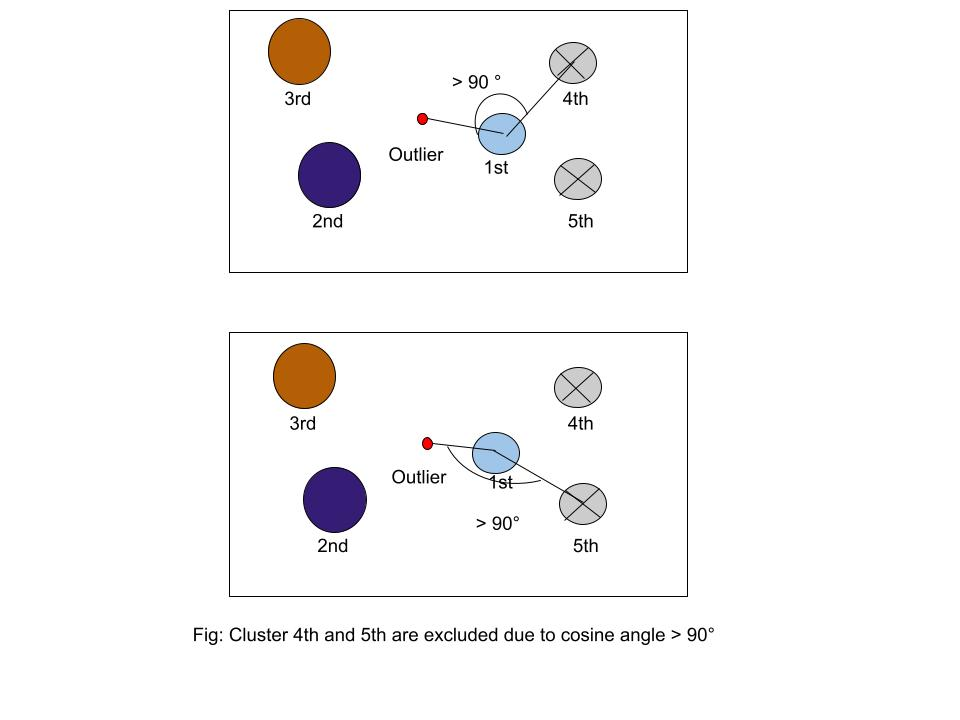
\includegraphics[scale=.5]{images/Copy of Object-inbet-instance.jpg}\\
Figure: Object in between clusters
\end{figure}
\noindent In the figure we have seen that the 4th and 5th clusters are not considered as neighboring clusters for the outlier. This is because both these clusters are behind of 1st cluster which is closer to the outlier. We have excluded them from the candidate neighbor cluster list by calculating the cosine distance with outlier with respect to 1st cluster which are $>1$. We have implanted this operation from lines 18 to 31 in our algorithm.\\
We have used python language and \textit{scipy} package in our algorithm where cosine distance $<1$ means the cosine angle is in between $cos90^0 $ and $-cos90^0$. And cosine distance $>1$ means the cosine angle is in between $cos90^0 $ and $cos270^0$. We have considered cosine distance $<1$ to find out a neighbor cluster of an outlier because it provides a convex surround cluster. Finally, we have got the nearest neighbor cluster of in-between instances by filtering the candidate cluster list that is implemented from lines 36 to 41 in our algorithm. We can reduce the value of cosine distance to get a more precise and opposite cluster. Here precise opposite cluster means if one cluster is located on one side of the outlier and another is located on the other side by almost $180^0$ angle. We can get a clear idea by looking at the following figure:
\begin{figure}[H]
\centering
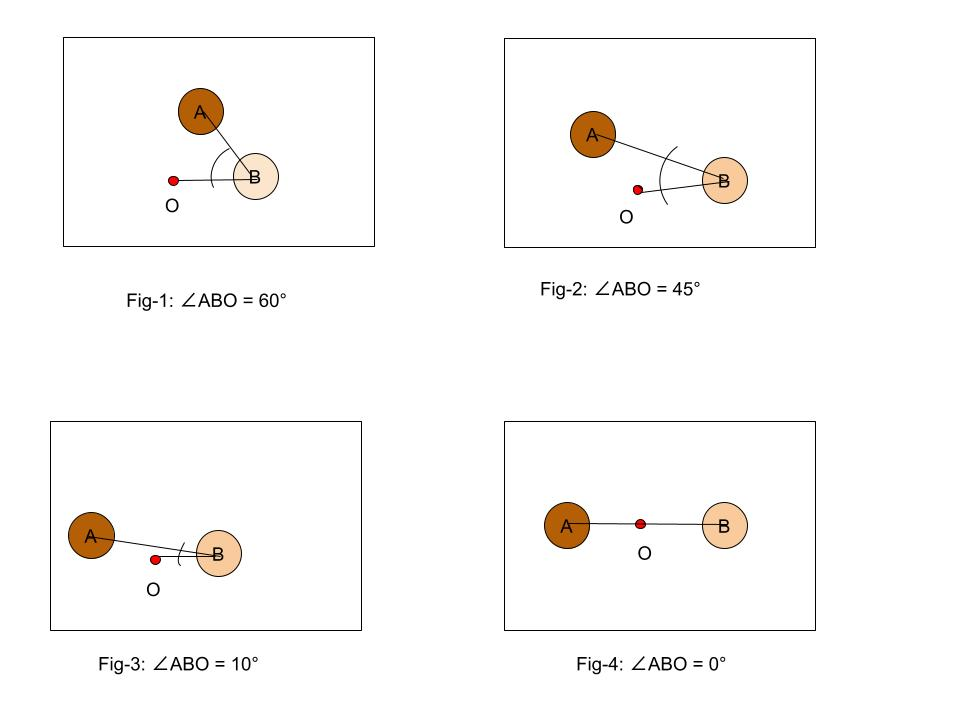
\includegraphics[scale=.5]{images/Opposite-cluster.jpg}\\
Figure: Reducing angle to get more opposite cluster
\end{figure}
\noindent Here in this figure, we can see that in the 1st sub-figure cluster-A and cluster-B are relatively on the same side from the outlier-o and the angle between the outlier-o and cluster-A is $60^0$ with respect to cluster-A. In the 2nd sub-figure, these 2 clusters are located on relatively opposite sides considering the outlier position where the cosine angle between outlier and cluster-A is $45^0$. And the next two subsequent figures we can see the more we decrease the cosine angle the more opposite cluster we can have.
% [(inbetweenobject,[neighclust1, neighclust5,...]),(),...]

\subsection{Challenges/Cases to take care of/insights}
To get our desired output we have faced several kinds of challenges which are given below:

\begin{itemize}
    \item First of all, We are looking for a data-set with some clusters and outliers. For that, we have decided to use \textit{K-means clustering algorithm} but we have realized that by applying \textit{K-means algorithm} we can not have an outlier. After that, We have decided to use \textit{Agglomerative clustering algorithm}. To define the distance threshold to cut a cluster we have applied this algorithm without a distance threshold and observed the dendrogram to select the distance threshold. After having the threshold, we again implanted this algorithm over the data-set with the computed distance threshold. As a result, we have got a set of clusters and outliers.
    
    \item After having a set of clusters we have found out k-nearest cluster for an outlier by euclidean distance. But we observed that all k-nearest clusters are not important to consider as a neighbor clusters of the outlier because some clusters are behind of other clusters. But we need those clusters that are directly faced by in-between instances. For that, we have considered the cosine distance between two clusters since the cosine similarity takes through the enclosed angle between (two) vectors also to some extent the geometry. If the cosine distance is less than 1 we have decided that one cluster is followed by other clusters. So which is closer than the other we have considered that and discarded the other one.

    \item After implementing our new approach to detect in-between instances to our synthetic data-set we did not get our desired output. Our new method was not able to discard those clusters that are behind other clusters. This made it necessary to identify the problem. We have discovered an error in our implementation.
    The root of the problem lies in the fact that while we are computing the cosine distance between two clusters, we are considering an origin at the null vector (0,0) in a Cartesian coordinate system. But it was supposed to consider our outlier as an origin. In order to be capable to determine what is behind another cluster we need to take the viewpoint from the perspective of an outlier, which requires the outlier to be considered as the center  / 'null point'. For that, we have geometrically translated our outlier to the origin and compensated other elements according to our new origin. Here with the term 'compensate' we refer to the necessity to not only translate our outlier but also other elements/objects in order to maintain the relative properties such as distances and angles between the objects.
    
    \item Unfortunately we didn't get our expected output yet. Actually, we need to calculate the cosine distance between an outlier and a cluster with respect to another cluster. This is because we are detecting whether a cluster is behind other clusters by considering the outlier. So we have translated a cluster to the origin(0,0) and calculated the cosine distance between the outlier and other clusters to decide whether they are behind or not of this origin cluster. Considering all the previous insights and improvements, the expected outcome/output is obtained. The journey sketched here shows that the geometry-oriented in-between instance detection is far away from being trivial.
\end{itemize}

%here you can sketch the "journey" from the first approach, what you expected to see, ...what you actually saw, ...why it was not as you expected, ....how you discovered the reason,....how you got the idea of how to 'fix it' / improve ....until finally you got an algorithm that yields the expected result of detecting properly in-between instances. :-)


\section{Evaluation}
Building on the previously presented and elaborated algorithm to detect in-between instances we owe some "proof" that convinces the reader of the effectiveness of the proposed method. For that purpose, we provide in this section several experiments. On different datasets, we apply our approach and inspect the results with the following question in mind: does our algorithm detect in-between instances and the enclosing clusters?

The experiments are conducted on artificial and real-world data. The artificial datasets bring the benefit of a controlled environment, allowing us to stress-test our approach on datasets/scenarios with specific properties. 
We have implemented our In-between instance over 3 different data-set. The first one is \textbf{Synthetic data-set}, the second one is \textbf{Consumer Complaint data-set} and the final one is \textbf{Molecular data-set}.
\subsection{Synthetic data-set}
We have created some synthetic data over 2d space to experiment with our algorithm. We can see the data distribution given below figure.
\begin{figure}[H]
\centering
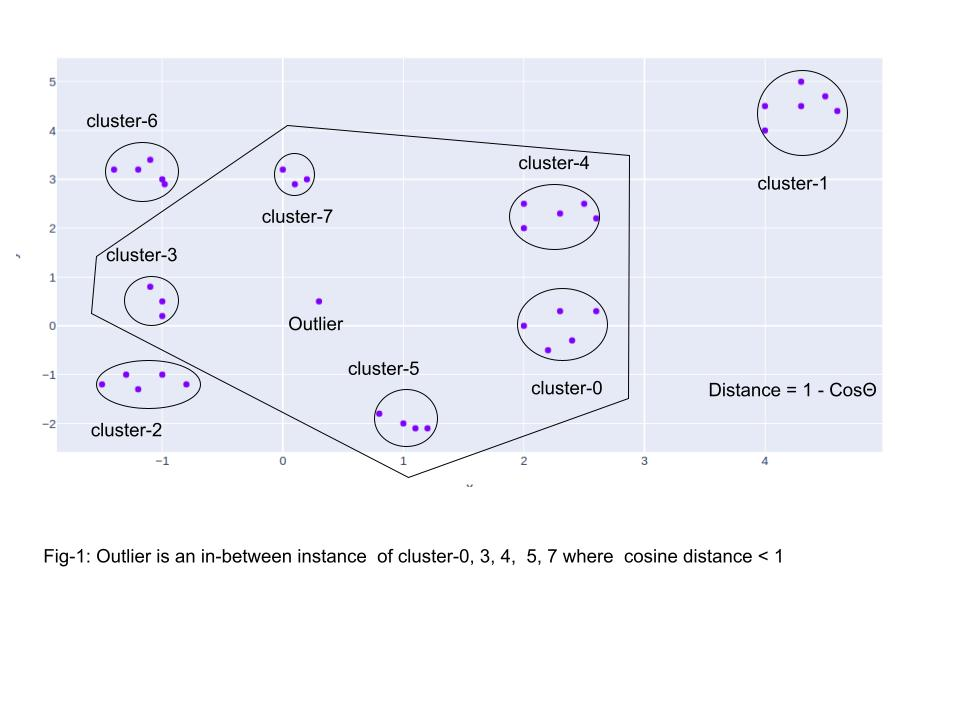
\includegraphics[scale=.5]{images/angle-1.jpg}\\
\end{figure}
\noindent Here we can see that there are eight clusters and one outlier where cluster-1 is behind cluster-4. Cluster-2 is also behind cluster-3 and cluster-6 is behind cluster-7. After implementing our 'In-between Instance' we have obtained cluster-0, 3, 4, 5, and 7  are neighbor clusters that are expected where we have considered the cosine distance less than 1.
\begin{figure}[H]
\centering
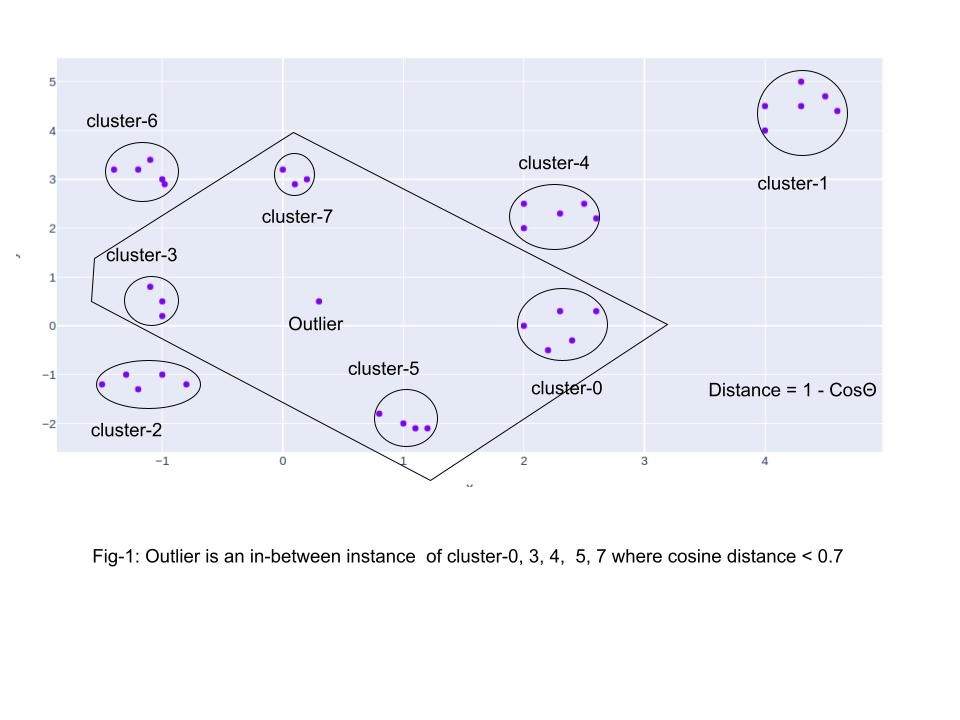
\includegraphics[scale=.5]{images/angle-.7.jpg}\\
\end{figure}
\noindent Here we can see that there are eight clusters and one outlier where cluster-1 is behind cluster-4. Cluster-2 is also behind cluster-3 and cluster-6 is behind cluster-7. After implementing our 'In-between Instance' we have obtained cluster-0, 3, 4, 5, and 7  are neighbor clusters that are expected where we have considered the cosine distance less than 1.
\begin{figure}[H]
\centering
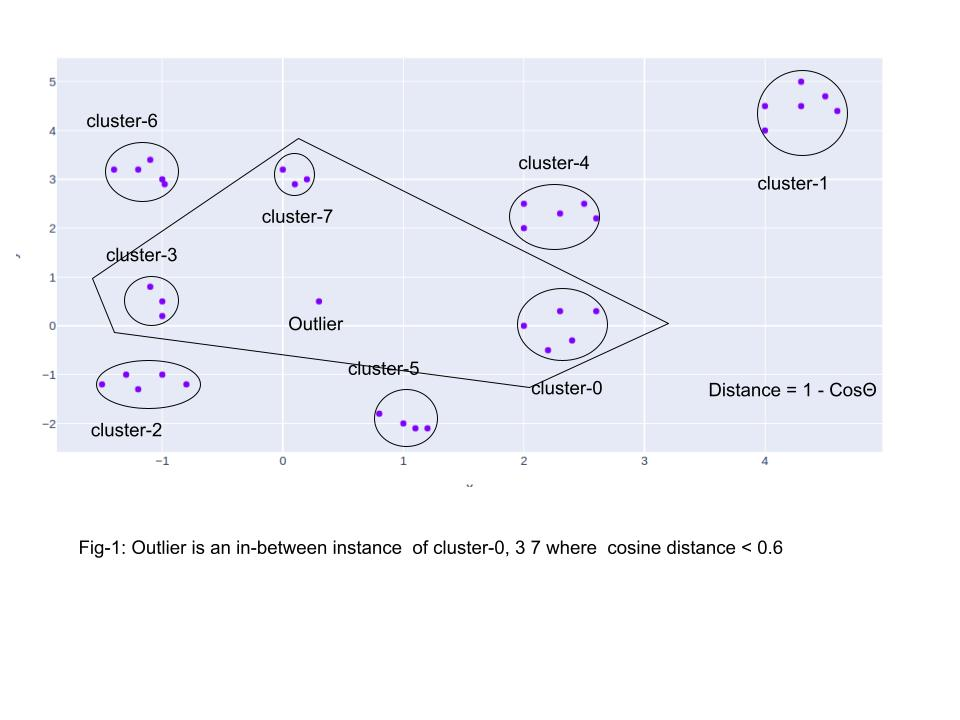
\includegraphics[scale=.5]{images/angle-.6.jpg}\\
\end{figure}
\noindent Here we can see that there are eight clusters and one outlier where cluster-1 is behind cluster-4. Cluster-2 is also behind cluster-3 and cluster-6 is behind cluster-7. After implementing our 'In-between Instance' we have obtained cluster-0, 3, 4, 5, and 7  are neighbor clusters that are expected where we have considered the cosine distance less than 1.
\begin{figure}[H]
\centering
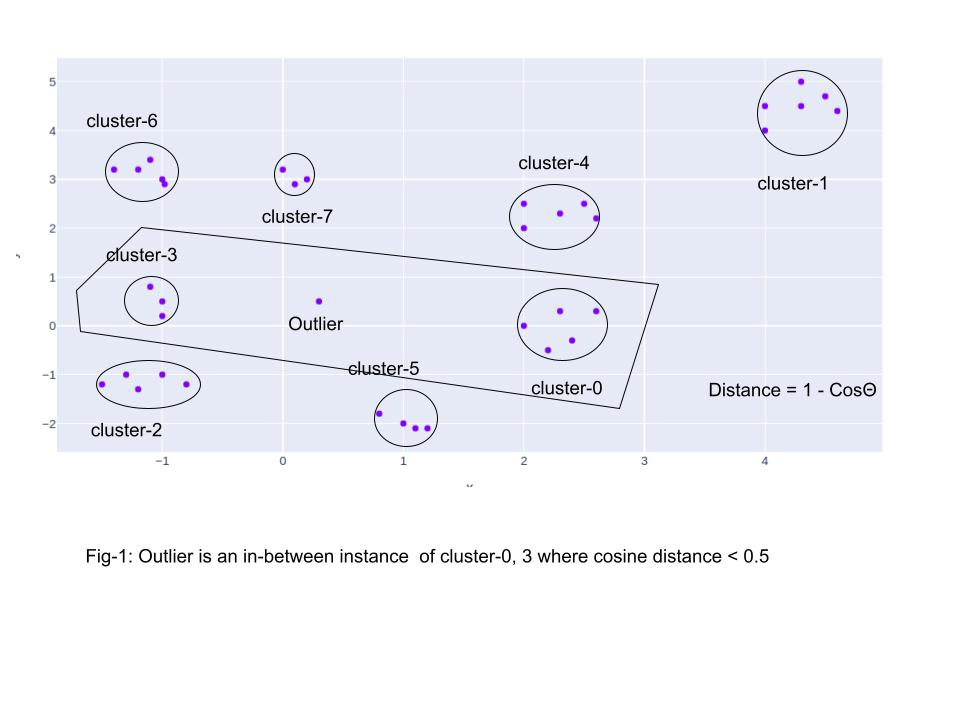
\includegraphics[scale=.5]{images/angle-.5.jpg}\\
\end{figure}
\noindent Here we can see that there are eight clusters and one outlier where cluster-1 is behind cluster-4. Cluster-2 is also behind cluster-3 and cluster-6 is behind cluster-7. After implementing our 'In-between Instance' we have obtained cluster-0, 3, 4, 5, and 7  are neighbor clusters that are expected where we have considered the cosine distance less than 1.

\begin{figure}[H]
\centering
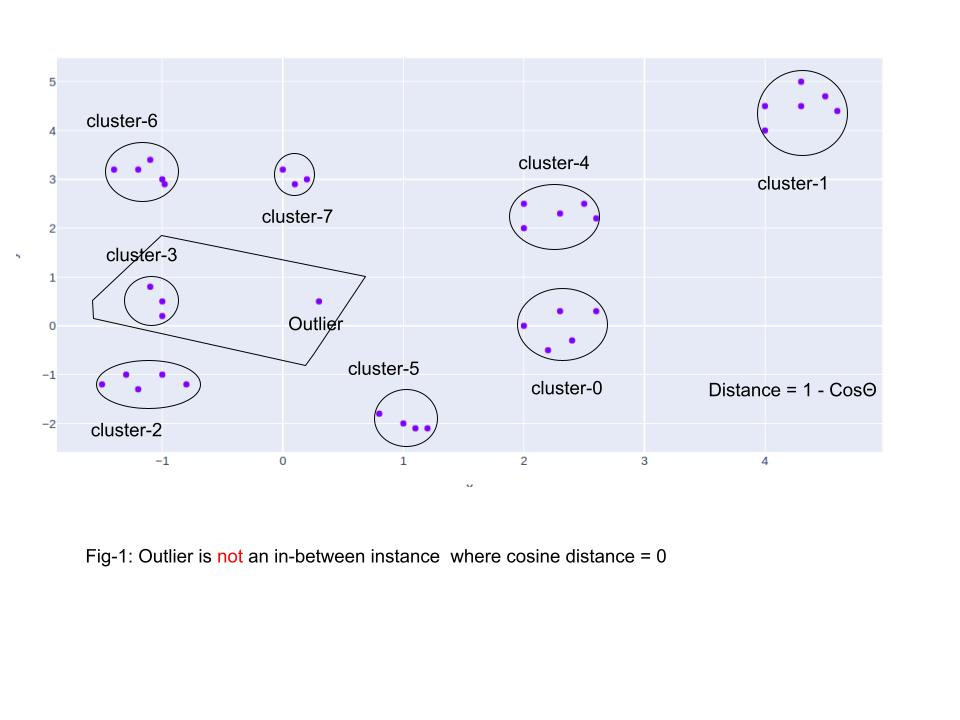
\includegraphics[scale=.5]{images/_ angle-.0.jpg}\\
\end{figure}
\noindent Here we can see that there are eight clusters and one outlier where cluster-1 is behind cluster-4. Cluster-2 is also behind cluster-3 and cluster-6 is behind cluster-7. After implementing our 'In-between Instance' we have obtained cluster-0, 3, 4, 5, and 7  are neighbor clusters that are expected where we have considered the cosine distance less than 1.\\
After seeing the output of our  algorithm implementation over the synthetic data set we have obtained a couple of observations which are:

\begin{itemize}
    \item the angle parameter is a sensitive parameter to obtain better output. Small changes in this parameter lead to great changes in the in-between instance detection. Because of the smaller angle, it prunes more clusters.
    \item we can see that there is an edge case. When we provide a very small angle near zero, there is a great possibility that we will not get an in-between instance. The ideal angle would be in the range of 40 - 70 degrees. Then we can have those clusters which are relatively far away from each other.
\end{itemize}
\subsection{Consumer Complaint data-set}
The Consumer Complaint Database is a collection of complaints about consumer financial products and services that we sent to companies for response. \\
The dataset contains different information on complaints that customers have made about multiple products and services in the financial sector, such as Credit Reports, Student Loans, Money Transfers, etc. This work is considered U.S. Government Work. The dataset is a public dataset and it was downloaded from https://catalog.data.gov/dataset/consumer-complaint-database
The date of each complaint ranges from November 2011 to May 2019.\\
The features/dimensions are:
\begin{figure}[H]
\centering
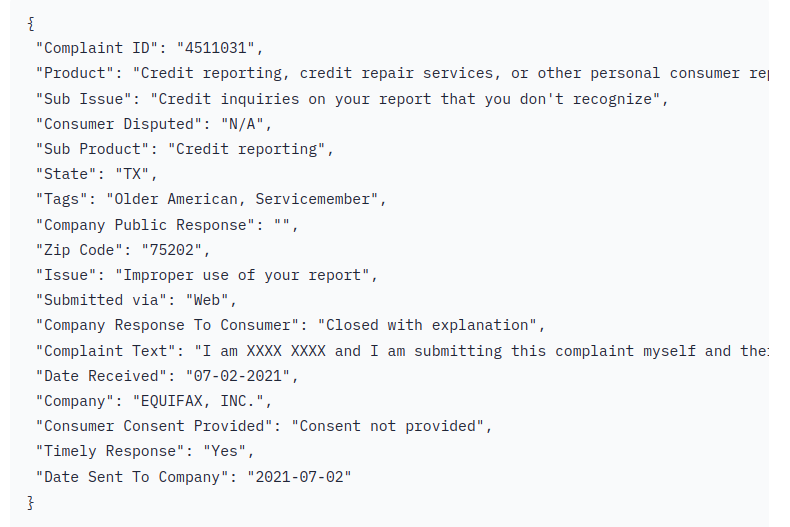
\includegraphics[scale=.55]{images/comlaint.png}\\
https://huggingface.co/datasets/consumer-finance-complaints-dataset-structure\\
Figure 4.2.1: Consumer-finance-complaints-dataset-structure
\end{figure}
\noindent We have considered \textbf{Complaint Text} features to cluster the dataset.
The text has been embedded using the method \textbf{doc2vec} embedding with 300 dimensions. 

After performing hierarchical clustering we obtain the following clusters (c.f. fig 4.2.2, i.e. a 2D projection of the high-dimensional (already clustered) data using t-SNE; with a remark that t-SNE is just for visualization and does not capture the geometry aka geometry is lost when using t-SNE).
\begin{figure}[H]
\centering
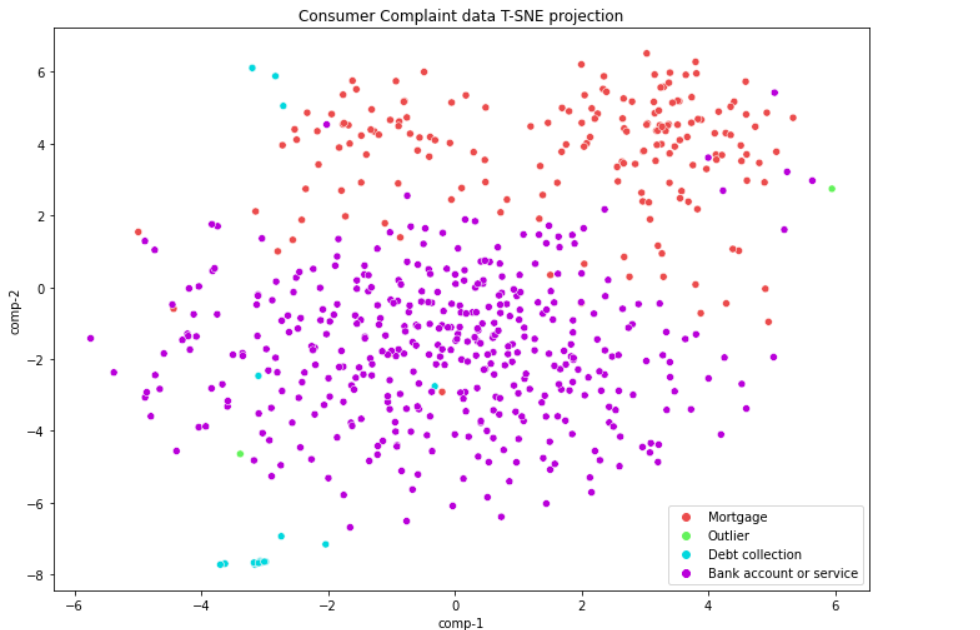
\includegraphics[scale=.55]{images/t-sne.png}\\
Figure 4.2.2: Consumer Complaint data T-SNE projection
\end{figure}
%https://scikit-learn.org/stable/modules/generated/sklearn.manifold.TSNE.html 

Taking a look at the single clusters (take those single clusters that are involved in an in-between instance) and identify 'qualitatively' what these complaints are roughly about (e.g. cluster 1 is about debt compensation, cluster 2 is about wrong data filled in the form ....). 

\begin{figure}[H]
\centering
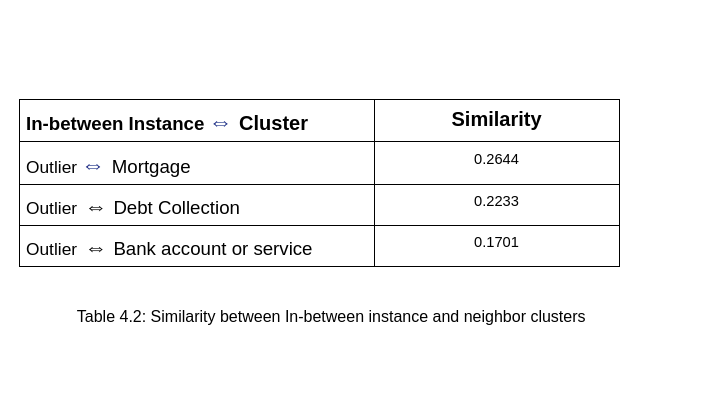
\includegraphics[scale=.6]{images/table-consumer.png}\\
\end{figure}

Then look at the in-between instance and identify pieces of it that are also visible in the single clusters.

\subsection{Molecular data-set}

The real-world example is based on a dataset compiled in \cite{mol2vec}

\begin{itemize}
    \item One does not need in the text data to know how the 300-dimensional objects actually lie behind each other (or to visualize it), but one knows, through the algorithm, that a particular cluster is 'behind' or 'in front' of another cluster or in-between instance
\end{itemize}

\section{Conclusion and Future Prospect}
Conclusion and Future Prospect

\newpage
\bibliographystyle{johd}
\bibliography{bib.bib}

\end{document}